% AI-transcribed component: printed 232--241.
% Principal PDF239--248; Google PDF243--252.
\begingroup
\clearpage
\noindent232\hfill\textsc{Trigonometrische Punktbestimmung.}\hfill\mbox{}\par\medskip
In Beziehung auf einen zweiten Punkt von bekannter Lage sollen $\varphi'$, $\alpha'$, $\beta'$, in Beziehung auf einen dritten $\varphi''$, $\alpha''$, $\beta''$, u.\,s.\,w. dasselbe bedeuten, was $\varphi$, $\alpha$, $\beta$ in Beziehung auf den ersten sind.

Sind die Winkelmessungen an dem zu bestimmenden Orte auf Einmal mit einem Theodolithen ohne Repetition gemacht, indem bei unverrücktem Instrument das Fernrohr nach der Reihe auf die verschiedenen bekannten Punkte geführt ist, so sollten, wenn $h$, $h'$, $h''$, u.\,s.\,w. die dabei abgelesenen Winkel bedeuten, die Ausdrücke
\[
\begin{gathered}
\varphi-h+\alpha\,\mathrm dx+\beta\,\mathrm dy\\
\varphi'-h'+\alpha'\mathrm dx+\beta'\mathrm dy\\
\varphi''-h''+\alpha''\mathrm dx+\beta''\mathrm dy\\
\text{u.\,s.\,w.}
\end{gathered}
\]
durch die Substitution der wahren Werthe von $\mathrm dx$ und $\mathrm dy$ alle einerlei Werth bekommen, wenn die Beobachtungen absolut genau wären; und wenn man also drei derselben unter sich gleich setzte, würde man durch Elimination die Werthe von $\mathrm dx$ und $\mathrm dy$ erhalten. Sind überhaupt nur drei bekannte Punkte beobachtet, so lässt sich auch nichts weiter thun; ist aber ihre Anzahl grösser, so werden die Fehler der Winkelmessungen am vollkommensten ausgeglichen, indem man alle obigen Ausdrücke addirt, die Summe mit der Anzahl dividirt, die Differenz zwischen diesem Quotienten und jedem einzelnen Ausdruck $=0$ setzt, und diese Gleichungen nach der bekannten Vorschrift der Methode der kleinsten Quadrate behandelt.

Sind hingegen die Winkelmessungen unabhängig von einander gemacht, so gibt jede derselben sofort eine Gleichung zwischen den unbekannten Grössen $\mathrm dx$ und $\mathrm dy$, und alle diese Gleichungen sind dann nach der Methode der kleinsten Quadrate zu combiniren, wobei man, wenn man will, auch noch auf die etwa ungleiche Zuverlässigkeit der Winkel Rücksicht nehmen kann. Wäre also z.\,B. der Winkel zwischen dem ersten und zweiten Punkte $=i$, zwischen dem zweiten und dritten $=i'$, u.\,s.\,w. gefunden, immer von der Linken zur Rechten gerechnet, so hätte man die Gleichungen
\[
\begin{gathered}
\varphi'-\varphi-i+(\alpha'-\alpha)\mathrm dx+(\beta'-\beta)\mathrm dy=0\\
\varphi''-\varphi'-i'+(\alpha''-\alpha')\mathrm dx+(\beta''-\beta')\mathrm dy=0\\
\text{u.\,s.\,w.}
\end{gathered}
\]

\clearpage
\noindent\mbox{}\hfill\textsc{Trigonometrische Punktbestimmung.}\hfill233\par\medskip
Haben diese Winkelmessungen gleiche Zuverlässigkeit, so bildet man aus diesen Gleichungen zwei Normalgleichungen, die erste, indem man jene der Ordnung nach mit den respectiven Coefficienten von $\mathrm dx$, d.\,i. die erste mit $\alpha'-\alpha$, die zweite mit $\alpha''-\alpha'$, u.\,s.\,w., multiplicirt und alles addirt; die andere, indem man dasselbe durch Multiplication mit den Coefficienten von $\mathrm dy$ ausführt und gleichfalls addirt. Ist hingegen die Winkelmessung von ungleicher Genauigkeit, und z.\,B. die erste auf $\mu$, die andere auf $\mu'$, u.\,s.\,w. Repetitionen gegründet, so müssen die Gleichungen beide Male vor der Addition auch erst noch mit diesen Zahlen $\mu$, $\mu'$, u.\,s.\,w. respective multiplicirt werden. Aus den so gefundenen beiden Normalgleichungen werden dann $\mathrm dx$ und $\mathrm dy$ durch Elimination gefunden. (Diese Vorschriften sind nur um derer willen beigefügt, denen die Methode der kleinsten Quadrate noch unbekannt ist, und für die vielleicht auch die Erinnerung noch nöthig sein könnte, dass bei jenen Multiplicationen die algebraischen Zeichen von $\alpha'-\alpha$, u.\,s.\,w. sorgfältig beachtet werden müssen.) Endlich bemerke ich noch, dass hiebei \textls[100]{nur} die Fehler der Winkelmessungen ausgeglichen werden sollen, indem die Coordinaten der bekannten Punkte als \textls[100]{genau} angesehen werden.

Ich erläutere diese Vorschriften für den zweiten Fall noch an den mir von Ihnen mitgetheilten Winkelmessungen auf der Holkensbastion bei Copenhagen, obwohl, wie es scheint; die zuletzt angezeigte Voraussetzung dabei nicht genau genug stattfindet; bei so kleinen Entfernungen haben kleine Unrichtigkeiten von einigen Zehntheilen eines Fusses in den gegebenen Coordinaten einen sehr viel grössern Einfluss, als die Fehler in den Winkelmessungen, und man darf sich daher nicht wundern, dass nach möglichster Ausgleichung der Winkel Differenzen zurückbleiben, die viel grösser sind, als bei den Beobachtungen der Winkel als möglich angenommen werden kann. Für den gegenwärtigen Zweck, wo nur ein Rechnungsbeispiel gegeben werden soll, kann dies jedoch gleichgültig sein.
\begin{center}
Winkel auf Holkensbastion\textsuperscript{*)}.
\end{center}
\begin{center}
\begin{tabular}{lrrr}
Friedrichsberg---Petri&$73^\circ$&$35'$&$22''{,}8$\\
Petri---Erlösersthurm&104&57&$33{,}0$
\end{tabular}
\end{center}
\vfill
\noindent\rule{4cm}{.4pt}\par
{\footnotesize *) Die Coordinaten der Punkte und die Winkel auf Holkensbastion beruhen beide auf Herrn Capit. v.~\textsc{Carocs} Messungen.\quad $S$\textit{[chumacher].}\par}
\medskip\noindent{\small IX.}\hfill30\hspace*{2cm}

\clearpage
\noindent234\hfill\textsc{Trigonometrische Punktbestimmung.}\hfill\mbox{}\par\medskip
\begin{center}
\begin{tabular}{lrrr}
Erlösersthurm---Friedrichsberg&$181^\circ$&$27'$&$5''{,}0$\\
Friedrichsberg---Frauenthurm&80&37&$10{,}8$\\
Frauenthurm---Friedrichsthurm&101&11&$50{,}8$\\
Friedrichsthurm---Friedrichsberg&178&11&$1{,}5$.
\end{tabular}
\end{center}
\begin{center}
Coordinaten, von der Copenhagener Sternwarte gerechnet, in Pariser Fuss.
\end{center}
\begin{center}
\begin{tabular}{lrr}
Petri&$+487{,}7$&$+1007{,}7$\\
Frauenthurm&$+710{,}0$&$+684{,}2$\\
Friedrichsberg&$+2430{,}6$&$+8335{,}0$\\
Erlösersthurm&$+2940{,}0$&$-3536{,}0$\\
Friedrichsthurm&$+3059{,}3$&$-2231{,}2$.
\end{tabular}
\end{center}
Als genäherte Coordinaten des Beobachtungsplatzes wurden angenommen:
\[
x=+2836{,}44,\qquad y=+444{,}33.
\]
Und damit fanden sich die Azimuthe:
\[
\begin{array}{lrrr@{\;}l}
\text{Petri}&166^\circ&30'&42''{,}56&+19{,}92\mathrm dx+83{,}04\mathrm dy\\
\text{Frauenthurm}&173&33&50{,}54&+10{,}80\mathrm dx+95{,}78\mathrm dy\\
\text{Friedrichsberg}&92&56&39{,}46&+26{,}07\mathrm dx+\phantom01{,}34\mathrm dy\\
\text{Erlösersthurm}&271&29&25{,}38&-51{,}79\mathrm dx-\phantom01{,}35\mathrm dy\\
\text{Friedrichsthurm}&274&45&41{,}39&-76{,}56\mathrm dx-\phantom06{,}38\mathrm dy.
\end{array}
\]
Der berechnete Winkel Friedrichsberg---Petri ist daher
\[
73^\circ34'3''{,}10-6{,}15\mathrm dx+81{,}70\mathrm dy,
\]
welches, mit dem beobachteten verglichen, die Gleichung
\[
-79{,}70-\phantom06{,}15\mathrm dx+\phantom081{,}70\mathrm dy=0
\]
gibt. Ebenso erhält man die fünf andern Gleichungen
\[
\begin{array}{r@{\;}r@{\;}r@{\;}l}
+69{,}82&-71{,}71\mathrm dx&-84{,}39\mathrm dy&=0\\
+9{,}08&+77{,}86\mathrm dx&+2{,}69\mathrm dy&=0\\
+0{,}28&-15{,}27\mathrm dx&+94{,}44\mathrm dy&=0\\
+0{,}05&-87{,}36\mathrm dx&-102{,}16\mathrm dy&=0\\
-3{,}43&+102{,}63\mathrm dx&+7{,}72\mathrm dy&=0.
\end{array}
\]
\clearpage
\noindent\mbox{}\hfill\textsc{Trigonometrische Punktbestimmung.}\hfill235\par\medskip
Aus der Verbindung dieser sechs Gleichungen erhält man, indem man den Beobachtungen gleiche Zuverlässigkeit beilegt, die beiden Normalgleichungen
\[
\begin{aligned}
+29640\mathrm dx+14033\mathrm dy&=+\phantom04170\\
+14033\mathrm dx+33219\mathrm dy&=+12384,
\end{aligned}
\]
und hieraus die Werthe
\[
\mathrm dx=-0{,}04,\qquad\mathrm dy=+0{,}39,
\]
oder die verbesserten Coordinaten der Holkensbastion
\[
+2836{,}40\quad\text{und}\quad+444{,}72.
\]
Die nach Substitution dieser Werthe von $\mathrm dx$ und $\mathrm dy$ zwischen den berechneten und beobachteten Winkeln zurückbleibenden Unterschiede sind noch viel zu gross, um den Messungen zugeschrieben werden zu können, und beweisen, was oben bemerkt ist, dass die Coordinaten der bekannten Punkte nicht auf Zehntheile des Fusses zuverlässig waren, weshalb denn freilich auch die gefundene Verbesserung selbst diesmal etwas zweifelhaft bleibt.

Die bei dieser Rechnung zum Grunde gelegten genäherten Coordinaten der Holkensbastion waren durch die \textls[100]{directe} Methode aus dem vierten und fünften der obigen Winkel berechnet. Obgleich diese directe Methode als ein ziemlich erschöpfter Gegenstand zu betrachten ist, so setze ich sie doch der Vollständigkeit wegen hier auch noch her, in derjenigen Gestalt, in welcher ich sie anzuwenden pflege.

Es seien $a$, $b$ die Coordinaten des ersten bekannten Punkts (man wählt denselben aus den drei bekannten nach Gefallen); die des zweiten seien in die Form
\[
a+R\cos E,\qquad b+R\sin E
\]
gebracht, und die des dritten in dieselbe:
\[
a+R'\cos E',\qquad b+R'\sin E'.
\]
Die gesuchten Coordinaten des Beobachtungspunkts bezeichne man durch
\[
a+\rho\cos\varepsilon,\qquad b+\rho\sin\varepsilon.
\]
Ferner sei der hier beobachtete Winkel zwischen dem ersten und zweiten
\vfill\noindent\hfill30\textsuperscript{$\ast$}\hspace*{2cm}

\clearpage
\noindent236\hfill\textsc{Trigonometrische Punktbestimmung.}\hfill\mbox{}\par\medskip
\noindent Punkte $=M$, der zwischen dem ersten und dritten $=M'$; ich setze voraus, dass diese Winkel von der Linken zur Rechten genommen, und dass sie, falls sie so über $180^\circ$ betragen haben, erst um $180^\circ$ vermindert sind, oder was dasselbe ist, dass, wenn ein Winkel in der verkehrten Ordnung unter $180^\circ$ betrug, statt seiner das Complement zu $180^\circ$ genommen ist\textsuperscript{*)}. Ich mache ferner
\[
\begin{array}{rcl@{\qquad}rcl}
\frac R{\sin M}&=&n,&\frac{R'}{\sin M'}&=&n'\\[5pt]
E-M&=&N,&E'-M'&=&N'
\end{array}
\]
(wo nöthigenfalls vorher $360^\circ$ addirt wird).

Dies vorausgesetzt, hat man die beiden Gleichungen
\[
\rho=n\sin(\varepsilon-N),\qquad\rho=n'\sin(\varepsilon-N'),
\]
welche, wenn sie so geschrieben werden:
\[
\frac1n=\frac1\rho\sin(\varepsilon-N),\qquad\frac1{n'}=\frac1\rho\sin(\varepsilon-N'),
\]
unter die Aufgabe Theor. Mot. C. C. p.~82 [**)] gehören. Die eine der dort gegebenen Auflösungen führt zu folgender Regel:

Ich nehme an, dass $n'$ grösser, wenigstens nicht kleiner, als $n$ ist, welches erlaubt ist, da es willkürlich ist, welchen Punkt man als den zweiten oder dritten betrachten will. Es sei
\[
\begin{gathered}
\frac n{n'}=\operatorname{tang}\zeta\\[5pt]
\frac{\operatorname{tang}\frac12(N'-N)}{\operatorname{tang}(45^\circ-\zeta)}=\operatorname{tang}\psi.
\end{gathered}
\]
Sodann wird
\[
\varepsilon=\tfrac12(N+N')+\psi,
\]
und nachdem $\varepsilon$ gefunden ist, wird $\rho$ durch eine der obigen Formeln, oder besser durch beide, berechnet.

In unserm Beispiele haben wir, den Frauenthurm als den ersten, Friedrichsberg vorläufig als den zweiten und den Friedrichsthurm als den dritten Punkt betrachtet:
\vfill
\noindent\rule{4cm}{.4pt}\par
{\footnotesize
*) Die Absicht davon ist, die folgenden Grössen $n$, $n'$ immer positiv zu machen, und dadurch weniger Aufmerksamkeit auf die algebraischen Zeichen nöthig zu haben.\par
[**) Band VII, Seite 100.]\par}

\clearpage
\noindent\mbox{}\hfill\textsc{Trigonometrische Punktbestimmung.}\hfill237\par\medskip
\[
\begin{array}{rcl@{\qquad}rcl}
a&=&+710{,}0&b&=&+684{,}2\\
E&=&77^\circ19'31''{,}91&E'&=&308^\circ51'45''{,}78\\
\log R&=&3{,}894\,4206&\log R'&=&3{,}573\,3549\\
M&=&99^\circ22'49''{,}20&M'&=&101^\circ11'50''{,}80\\
\multicolumn{3}{c}{\text{(zufolge obiger Anm.)}}&&&\\
N&=&337^\circ56'42''{,}71&N'&=&207^\circ39'54''{,}98\\
\log n&=&3{,}900\,2671&\log n'&=&3{,}581\,7019.
\end{array}
\]
Da hier $n>n'$, so vertauschen wir die Ordnung und setzen
\[
\begin{array}{rcl@{\qquad}rcl}
N&=&207^\circ39'54''{,}98&N'&=&337^\circ56'42''{,}71\\
\log n&=&3{,}581\,7019&\log n'&=&3{,}900\,2671.
\end{array}
\]
Hienächst findet sich ferner
\[
\zeta=25^\circ39'3''{,}49,\qquad
\psi=80^\circ45'31''{,}50,\qquad
\varepsilon=353^\circ33'50''{,}34
\]
und $\log\rho=3{,}330\,3996$, und die Coordinaten der Holkensbastion: $+2836{,}444$ und $+444{,}327$.
\vspace{1cm}
\begin{center}\rule{4cm}{.4pt}\end{center}

\clearpage
\noindent238\hfill\textsc{Nachlass.}\hfill\mbox{}\par
\vspace{1.5cm}
\begin{center}{\Large\textls[150]{NACHLASS.}}\end{center}
\bigskip
\begin{center}[7.]\\[5pt]
[Bestimmung der Lage des Punktes X durch Beobachtung der Winkel $\alpha$ und $\beta$ zwischen 3 gegebenen Punkten $A$, $B$, $C$.]
\end{center}
[Aus
\[
\frac{BA}{BX}.\frac{BX}{BC}.\frac{BC}{BA}=1
\]
folgt
\[
\frac{\sin XCB}{\sin BAX}=\frac{\sin C}{\sin A}=\frac{c\sin\beta}{a\sin\alpha}\,\bigg]
\]
\begin{center}
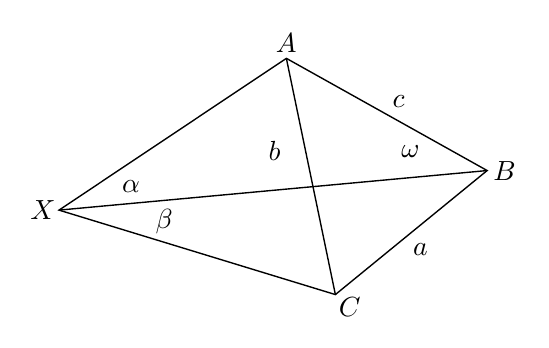
\begin{tikzpicture}[x=.75cm,y=.75cm,line width=.5pt]
\coordinate (X) at (0,0);
\coordinate (A) at (3.85,2.57);
\coordinate (B) at (7.25,.67);
\coordinate (C) at (4.68,-1.43);
\draw (X)--(A)--(B)--(C)--cycle;
\draw (X)--(B) (A)--(C);
\node[above,inner sep=2pt] at (A) {$A$};
\node[right,inner sep=2pt] at (B) {$B$};
\node[below right,inner sep=1pt] at (C) {$C$};
\node[left,inner sep=1pt] at (X) {$X$};
\node at (1.22,.40) {$\alpha$};
\node at (1.78,-.19) {$\beta$};
\node at (3.65,1.00) {$b$};
\node at (5.75,1.84) {$c$};
\node at (5.95,1.00) {$\omega$};
\node at (6.12,-.66) {$a$};
\end{tikzpicture}
\end{center}
[Setzt man
\[
\begin{gathered}
180^\circ-A=]\ \alpha+\omega=\lambda,\qquad [C=360^\circ-(A+\varepsilon),]\\
\alpha+\beta+B=\varepsilon\\[5pt]
\operatorname{tang}\varphi=\sqrt{\frac{c\sin\beta}{a\sin\alpha\cos\varepsilon}},
\end{gathered}
\]
dann ist
\[
\begin{gathered}
\operatorname{tang}\lambda=\operatorname{tang}\varepsilon\cos\varphi^2,\\
BX=\frac{c\sin\lambda}{\sin\alpha}.
\end{gathered}
\]
\clearpage
\noindent\mbox{}\hfill\textsc{Trigonometrische Punktbestimmung.}\hfill239\par\medskip
\begin{center}[8.]\\[5pt]Orientirung des Messtisches.\rlap{\hspace{.12em}\raisebox{1.15ex}{\scriptsize,}}\end{center}
Drei Örter $A$, $B$, $C$ sind auf dem M[ess]t[isch] durch $a$, $b$, $c$ vorgestellt; die geraden Linien $Aa$, $Bb$, $Cc$ schneiden einander in den Punkten $\alpha$, $\beta$, $\gamma$.

In $b$ auf $ab$ und in $\gamma$ auf $a\gamma$ errichtete Senkrechte schneiden einander in $e$; in $c$ auf $ac$ und in $\beta$ auf $a\beta$ Senkrechte schneiden einander in $f$; man verbinde $e$ und $f$ und fälle darauf aus $a$ das Perpendikel $aM$. So ist $M$ auf dem Messtisch der Standpunkt.
\bigskip
\begin{center}[9.]\\[5pt]Aufgabe der praktischen Geometrie.\end{center}
$A$, $B$, $C$, $D$ sind vier Punkte in einer horizontalen Ebene; $B$, $C$, $D$ liegen in gerader Linie und
\[
BC=CD.
\]
Es seien die Azimuthe der Linien
\[
\begin{array}{l@{\;}l}
DB\ .\ .\ .\ .&f\\
AB\ .\ .\ .\ .&f+g-\delta\\
AC\ .\ .\ .\ .&f+g-x\\
AD\ .\ .\ .\ .&f+g+\delta.
\end{array}
\]
\begin{center}
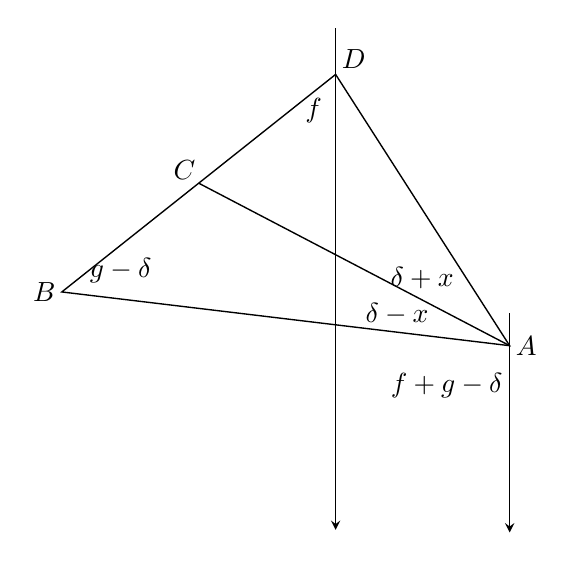
\begin{tikzpicture}[x=.65cm,y=.65cm,line width=.5pt]
\coordinate (B) at (0,0);
\coordinate (D) at (5.35,4.25);
\coordinate (C) at (2.675,2.125);
\coordinate (A) at (8.75,-1.05);
\draw (B)--(D)--(A)--cycle;
\draw (C)--(A);
\draw[->,>=stealth] (5.35,5.15)--(5.35,-4.65);
\draw[->,>=stealth] (8.75,-.42)--(8.75,-4.7);
\node[left,inner sep=2pt] at (B) {$B$};
\node[above left,inner sep=1pt] at (C) {$C$};
\node[above right,inner sep=2pt] at (D) {$D$};
\node[right,inner sep=2pt] at (A) {$A$};
\node at (1.15,.42) {$g-\delta$};
\node at (4.92,3.55) {$f$};
\node at (7.04,.28) {$\delta+x$};
\node at (6.55,-.44) {$\delta-x$};
\node at (7.52,-1.83) {$f+g-\delta$};
\end{tikzpicture}
\end{center}

\clearpage
\noindent240\hfill\textsc{Bemerkungen.}\hfill\mbox{}\par\medskip
\[
\bigg[\frac{AC}{BC}=\frac{AC}{CD}\quad\text{oder}\quad
\frac{\sin(g-\delta)}{\sin(\delta-x)}=\frac{\sin(g+\delta)}{\sin(\delta+x)}.\bigg]
\]
Sodann ist
\[
\begin{gathered}
\operatorname{tang}x=\frac{\operatorname{tang}\delta^2}{\operatorname{tang}g},\\[6pt]
\sin x=\frac{\sin\delta^2\cos(g-x)}{\sin g},
\end{gathered}
\]
oder proxime
\[
x=206265''\sin\delta^2\operatorname{cotang}g.
\]
\bigskip
\begin{center}\rule{3cm}{.4pt}\\[6pt]\textsc{Bemerkungen.}\end{center}
\begingroup\footnotesize
Die Notizen [1] und [9], [3] und [4], sowie [8] wurden 3 verschiedenen Handbüchern entnommen; [2] und [7] sind auf die letzten Seiten von Logarithmentafeln eingetragen; [5] entstammt einem Rechnungsblatte zur hannoverschen Gradmessung.

Die Formeln des Art.~[2], die auch bei Art.~[3] benutzt sind, lassen sich wie folgt ableiten. Es seien $x$, $y$ die Coordinaten des zu bestimmenden Punktes; $x_0$, $y_0$ die Coordinaten für eine genäherte Lage desselben; $a$, $b$, $a'$, $b'$, $a''$, $b''$ die Coordinaten der Beobachtungsplätze; $r$, $r'$, $r''$ die Entfernungen dieser Plätze vom Punkte $(x_0,y_0)$. Dann erhält man durch Differentiation der Gleichung
\[
\operatorname{tang}(A+\alpha)=\frac{y_0-b}{x_0-a},
\]
indem man $\mathrm dx_0=x-x_0$, $\mathrm dy_0=y-y_0$, $A+\alpha+\mathrm d(A+\alpha)=A+\delta A$ setzt, die Fehlergleichung:
\[
\delta A-\alpha=-\sin A.\frac{x-x_0}{r}+\cos A.\frac{y-y_0}{r}.
\]
Ebenso ergibt sich
\[
\delta A'-\alpha'=-\sin A'.\frac{x-x_0}{r'}+\cos A'.\frac{y-y_0}{r'}
\]
und
\[
\delta A''-\alpha''=-\sin A''.\frac{x-x_0}{r''}+\cos A''.\frac{y-y_0}{r''}.
\]
Eliminirt man $x-x_0$, $y-y_0$, so entsteht die Bedingungsgleichung:
\[
r\sin(A'-A'').(\delta A-\alpha)+r'\sin(A''-A).(\delta A'-\alpha')+r''\sin(A-A').(\delta A''-\alpha'')=0
\]
oder
\[
l.\delta A+l'.\delta A'+l''.\delta A''=l\alpha+l'\alpha'+l''\alpha''.
\]
Macht man nun mit Rücksicht hierauf
\[
g.\delta A^2+g'.\delta A'^2+g''.\delta A''^2\quad\text{zum Minimum},
\]
so wird
\par\endgroup

\clearpage
\noindent\mbox{}\hfill\textsc{Trigonometrische Punktbestimmung.}\hfill241\par\medskip
\begingroup\footnotesize
\[
\delta A=\frac{lk}{g},\qquad\delta A'=\frac{l'k}{g'},\qquad\delta A''=\frac{l''k}{g''};
\]
\[
k=\frac{l\alpha+l'\alpha'+l''\alpha''}{\dfrac{ll}{g}+\dfrac{l'l'}{g'}+\dfrac{l''l''}{g''}}.
\]
Hienach ist
\[
y-b=(x-a)\operatorname{tang}(A+\delta A)=(x-a)\operatorname{tang}A+\frac{r.\delta A}{\cos A}
=(x-a)\operatorname{tang}A+\frac{rlk}{g\cos A}.
\]
In dem Zahlenbeispiel unter [3] sind einige kleine Fehler berichtigt worden, wodurch hier die Werthe der Coordinaten für York etwas abweichend von den im Coordinatenverzeichnisse, Band IV, S.~436, angegebenen Werthen erhalten wurden.

Ebenso ist in dem unter [5] aufgeführten Beispiele für Vorwärtseinschneiden ein kleines Versehen richtig gestellt worden. Die beobachteten Azimuthe auf den festen Punkten und die Coordinaten sind auch in den »Abrissen u.\,s.\,w.«, Band IV, S.~454, 456 und 457, angegeben.

Zur Bestimmung von Nebenpunkten wurde von \textsc{Gauss} sowie von den ihm beigegebenen Officieren gewöhnlich das Verfahren des Art.~[5] angewandt. Die Rechnungen dafür sind aber fast ganz allein von \textsc{Gauss}, und zwar in der angegebenen Weise, ausgeführt worden. In dem Arbeitsbericht für 1830 an das hannoversche Ministerium heisst es: »Bei der hiesigen trigonometrischen Vermessung habe ich bisher diesen Theil des Geschäfts [Verarbeitung der Messungen zu Resultaten] ganz allein auf mich genommen. Meine Berichte über die Arbeiten von 1828 und 1829 geben eine Uebersicht über den Umfang des in diesen Jahren geleisteten. Ohne hier in umständliche Details einzugehen, darf ich doch nicht unbemerkt lassen, dass mir die Verarbeitung nur dadurch möglich geworden ist, dass ich ihr meine \textls[100]{ganze} mir von meinen unmittelbaren Dienstgeschäften gebliebene Zeit gewidmet habe.« Und in dem am 8.~Februar 1838 erstatteten Bericht an das Ministerium sagt \textsc{Gauss}: »Zu einer trigonometrischen Messung sind zweierlei ganz verschiedenartige Arbeiten erforderlich, die Ausführung der Messungen an den betreffenden Plätzen im Felde, und ihre Verarbeitung zu Resultaten durch Combination und Calcül im Zimmer. Den zweiten Theil des Geschäfts habe ich bisher ganz auf mich selbst genommen.« Nur zwei Monate des Winters 1830/31 hat ihn sein Sohn, der Lieutenant J.~\textsc{Gauss}, dabei unterstützt; in den letzten Jahren der hannoverschen Landesvermessung scheint auch Professor \textsc{Goldschmidt} geholfen zu haben. Einem von diesem ausgearbeiteten »geodätischen Calcül nach \textsc{Gauss}« aus dem Jahre 1835, der eine »kurze Darstellung nach von \textsc{Gauss} gegebenen Privatmittheilungen« bieten will, sind die nachstehenden Ausführungen entnommen:

»Bei der Festsetzung der Nebenpunkte fangen wir damit an, diejenigen zu bestimmen, welche sich aus den Hauptdreieckspunkten allein \textls[100]{scharf} bestimmen lassen, so dass 1) die Richtungen sich nicht unter zu spitzen Winkeln schneiden und 2) man gewiss ist, dass die angeführten Azimuthe sich wirklich auf den Punkt quaestionis beziehen, indem es bei ausgedehnten Operationen leider nur zu häufig vorkommt, dass eine Namensverwechselung stattfindet. Hat man indessen den Punkt aus mehr als 2 Hauptpunkten bestimmt, oder auf dem Punkte selbst gemessen, so kann eine solche Verwechselung nicht wohl stattfinden. So setzt man nun diese Nebenpunkte fest, indem man, wenn man scharfe Resultate haben will, nicht nur alle Hauptdreieckspunkte, sondern auch die nach und von andern schon bestimmten Nebenpunkten gemachten Schnitte mit hinzuzieht. Es entstehen dabei 3 unbekannte Grössen, die Coordinaten des Punktes und die daselbst stattfindende Orientirung. Man berechnet nun auch diese Elemente für die übrigen Nebenpunkte. Sollte vielleicht es nachher noch für gut gefunden werden, neue Nebenpunkte einzuführen, indem es vielleicht bei der anfänglichen Disposition übersehen wurde, dass dieses Einführen rathsam wäre, so hat man doch nicht nöthig, sich auf diejenigen Stationen zu begeben, von denen ab die neuen
\par\endgroup
\vfill\noindent{\small IX.}\hfill31\hspace*{2cm}
\endgroup
% Continues on printed 242 with "Punkte geschnitten werden könnten".
